\documentclass[10pt,conference,compsocconf]{IEEEtran}

\usepackage{url}
\usepackage{xcolor}
\usepackage{eurosym}
\usepackage{amsfonts}
\usepackage{balance}
\usepackage[pdftex]{graphicx}
   %declare the path(s) where your graphic files are
  % and their extensions so you won't have to specify these with
 % every instance of \includegraphics
\DeclareGraphicsExtensions{.pdf,.jpg,.png}

\hyphenation{second-ly ap-pen-dix}

\clubpenalty = 10000
\widowpenalty = 10000
\displaywidowpenalty = 10000

\newcommand{\todo}[1]{\textbf{#1}}

\begin{document}
%
% paper title
% can use linebreaks \\ within to get better formatting as desired
\title{End-User Refactoring}

\author{\IEEEauthorblockN{Felienne Hermans, David Hoepelman}
\IEEEauthorblockA{Delft University of Technology\\
Mekelweg 4\\
2628 CD Delft, the Netherlands\\
f.f.j.hermans@tudelft.nl}


\and
\IEEEauthorblockN{Katryn Stolee}
\IEEEauthorblockA{Iowa State University\\
209 Atanasoff Hall\\
Ames, IA 50011-1041\\
Email Katie}
}

\maketitle

\begin{abstract}
\end{abstract}


\begin{IEEEkeywords}
end-user computing; refactoring; 
\end{IEEEkeywords}

\section{Introduction}
The number of end-user programmers is said to greatly exceed the number of professional programmers. ``The proportion of American end user workers reporting they “do programming” has remained relatively constant, rising from around 10\% in 1989 to only around 15\% in 2001''~\cite{Scaf2005} This 15\% of 2001 totals to about 11 million end users, while the number of professional developers was estimated at 3 million for the same period~\cite{Scaf2005}.

These end-user programmers perform a wide variety of tasks within the organizations they work for, ranging from building or maintaining applications to simple data manipulation in a spreadsheet. While performing these tasks, end-users user programmers face many of the challenges of professional developers, such as identifying faults, debugging, or understanding someone else’s code~\cite{Ko2011}.

Contrary to what people might think, end-user artifacts are not always created ad-hoc, but may in fact have a long life-span. A recent case study showed that spreadsheets have an average lifespan of 5 years~\cite{Hermans2011}. In their lifespan, these artifacts are modified, often by different people. This makes them vulnerable for \emph{smells}, like programming artifacts. 

These smells in end-user programming have been a topic of research over the past few years. Most notable are smells in Yahoo Pipes~\cite{Stolee2011}, smells in spreadsheets\todo{cite}, and performance smells in Labview code\todo{cite}. Experiments in all these areas have shown that end-users in fact understand smells and often prefer versions of their code that are non-smelly. Alleviating those smells can be achieved with refactoring, which leads us to the topic of this paper: how can we support do end-users in refactoring their artifacts? \todo{This is up for discussion.}

\section{Background}
\label{sec:background}
Since there introduction by Martin Fowler in 1999, extensive research has been done into code smells. Code smells, according to Fowler, indicate suspicious or weak parts parts, that the developer might want to change, in order to improve readability and minimize the chance of future errors~\cite{Fowl1999} `'A code smell is a surface indication that usually corresponds to a deeper problem in the system'', says Fowler. Just as source code produced by professionals, end-user program can also contain smells.

\section{Smells in end-user artifacts}
\label{sec:smells}
Research into end-user programming smells comes in two different variants. Some authors have interviewed end-users to obtain an understanding of smells perceived by them \todo{cite Labview}. Other authors have taken Fowler's smells and transformed them slightly to be applicable to end-user artifacts~\cite{Hermans2012,Hermans2012-2}. There are also authors~\cite{Stolee2011} that have combined these two approaches. This section provides an overview of different types of smells that can be applicable to end-user artifacts.

\subsection{Smells in spreadsheets}
Fowler defines his smells on two levels: within classes and between them. This is a distinction that can be easily translated to spreadsheets: smells within worksheets and smells between them. In \cite{Hermans2012-2}, Hermans \emph{et al.} describe \emph{inter-worksheet} smells and in \cite{Hermans2012} they add smells within worksheets.
\todo{more summary here}

\subsection{Smells in Labview code}
\todo{add summary here}

\subsection{Smells in Yahoo pipes}
In ~\cite{Stolee2011}, Stolee and Elbaum describe a number of smells. In addition to the smells, they present evidence that users of Yahoo pipes prefer non-smelly pipes over smelly ones, as shown in Figure \ref{fig:Table1-Stolee2011}.

\begin{figure}[ht!]
\centering
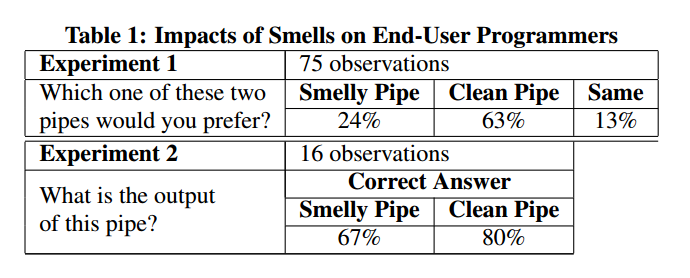
\includegraphics[width=\columnwidth]{Table1-Stolee2011.png}
\caption{End-users showing a preference for non-smelly pipes(from \cite{Stolee2011})}
\label{fig:Table1-Stolee2011}
\end{figure}

\todo{more summary here}

\section{Refactoring end-user programs}
\label{sec:refactoring}
Now that we have described various smells in different end-user artifacts, we direct our attention to the refactoring of them. 

\section{Empirical evidence}
\label{sec:empirical}


\section{Related Work}
\label{sec:related_work}

\section{Discussion}
\label{sec:discussion}


\section{Concluding Remarks}
\label{sec:conclusions}



\newpage
\balance
\bibliographystyle{plain}
\bibliography{literaturelist}

\end{document}


